\documentclass{thesis}%
\usepackage[T1]{fontenc}%
\usepackage[utf8]{inputenc}%
\usepackage{lmodern}%
\usepackage{textcomp}%
\usepackage{lastpage}%
\usepackage{graphicx}%
\usepackage{caption}%

 
\renewcommand{\listfigurename}{Seznam obrázků}
\captionsetup[table]{name=Tabulka}
\captionsetup[figure]{name=Obr.}
\renewcommand\listtablename{Seznam tabulek}
\renewcommand{\contentsname}{Obsah}
\renewcommand{\refname}{Seznam zdrojů}


\begin{document}%
\tableofcontents
\newpage

\chapter{Úvod}
Počítačové vidění je rychle se rozvíjející oblastí kybernetiky, která pomáhá v různých aplikacích. Hlavním cílém této oblasti je rozpoznávání obrazu respektive získavání informací ze zachycených obrazů.
Ty je pak možné použít například v oblasti automatizace průmyslu pro autonomní průmyslové roboty, detekci jevů například v bezpečnostním kamerovém systému, interakci člověka s počítačem či k realizaci
autonomního řízení automobilů. Počítačové vidění nachází často uplatnění i v oblasti medicíny, kde je možné automaticky pomocí software ze získáaných medicínských dat a snímků provádět například automatickou
diagnózu.\\
Díky velkému množství zobrazovacích metod využiváných v oblasti medicíny a díky moderním technikám počítačového vidění je možné usnadnit lékařům diagnózu a to často s využitím kombinace několika
zobrazovacích metod.\\
\subsection{Zobrazovací metody v medicíně}
Zobrazovací metody jsou definován ve Velkém lékařském slovníku následovně:
lékařské vyšetřovací metody umožňující zobrazení orgánů a jejich částí v živém organismu bez narušení jejich životnosti. Kromě vlastního zobrazení struktury umožňují mnohé moderní metody i posouzení funkčního stavu. Z. m. využívají různých fyzikálních principů a k jejich rozvoji přispěl mj. i rozvoj počítačové techniky. K hlavním metodám patří rentgenové vyšetření v mnoha modifikacích vč. CT, ultrazvukové vyšetření ultrasonografie, magnetická rezonance MRI, izotopová vyšetření, PET aj. Zocor – simvastin, hypolipidemikum ze skupiny statinů)\cite{hugo}\\


\subsection{Rentgen}
Rentgenové záření \footnote[1]{Rentgenové zářeí objevil v roce 1895 německý fyzik W. C. Röntgen behěm studia výbojů v plynech}- elektromagnetické záření o velmi krátké vlnové délce 10nm - 0,001nm. Pokud je vlnová délka rentgenového záření velmi malá pak hovoříme a tvrdém rentgenovém záření, které má vyšší energie. Nižší energii pak mmá zcela logicky záření nazývané jako měkké má vetší vlnovou délku.
\subsubsection{Princip vzniku rentgenového záření}
Při dopadu katodového záření - proudu elektronů, které jsou urychleny elektrickým polem na kovovou anodu dochází ke vzniku záření, které proniká i neprůhlednými předměty. Jako důsledek zpomalování pohyu elektronů dopadajících velkou rychlostí na anodu, dochází kevzniku tzv. brzdného záření. Spektrum brzdného záření je spojité, jako důsledek spojitých změn frekvence. Dalším zářením, které vzniká je tzv. charakteristické záření, které ji získaly působením dopadajících elektron. V tomto případě pozorujeme čárové spektrum.
\subsection{Výpočetní tomografie CT}
Výpočetní tomografie je metodou využívající matematické rekonstrukce obrazu získaného sérií rentgenových snímků. Pomocí této metody je možné regresivním způsobem zobrazovat měkké tkáně jako jsou například ledviny, svalstvo, mozek nebo další orgány jako jsou například játra. Touto metodou je možné zjistit patologické jevy, které se liší svou denzitou od okolní tkáně nebo okolí obecně.
\subsubsection{Historie CT}
Historie výpočetní tomografie sahá do roku 1963, kdy Allan Cormack (americký fyzik) vypracoval teorii o rekonstrukci tomografického řezu z několika sumačních snímků. V této teorii využil Allan Cormack gama záření. První skutečně použitelný tomograf byl však sestroj o necelých deset let později a to v roce 1972. Sestavil jej Godfrey Newbold Hounsfield. \footnote[2]{Allan Cormack a  Godfrey Newbold Hounsfield obdrželi za své objevy v roce 1979 Nobelovu cenu.} \\
\begin{figure}[h]
 \centering
	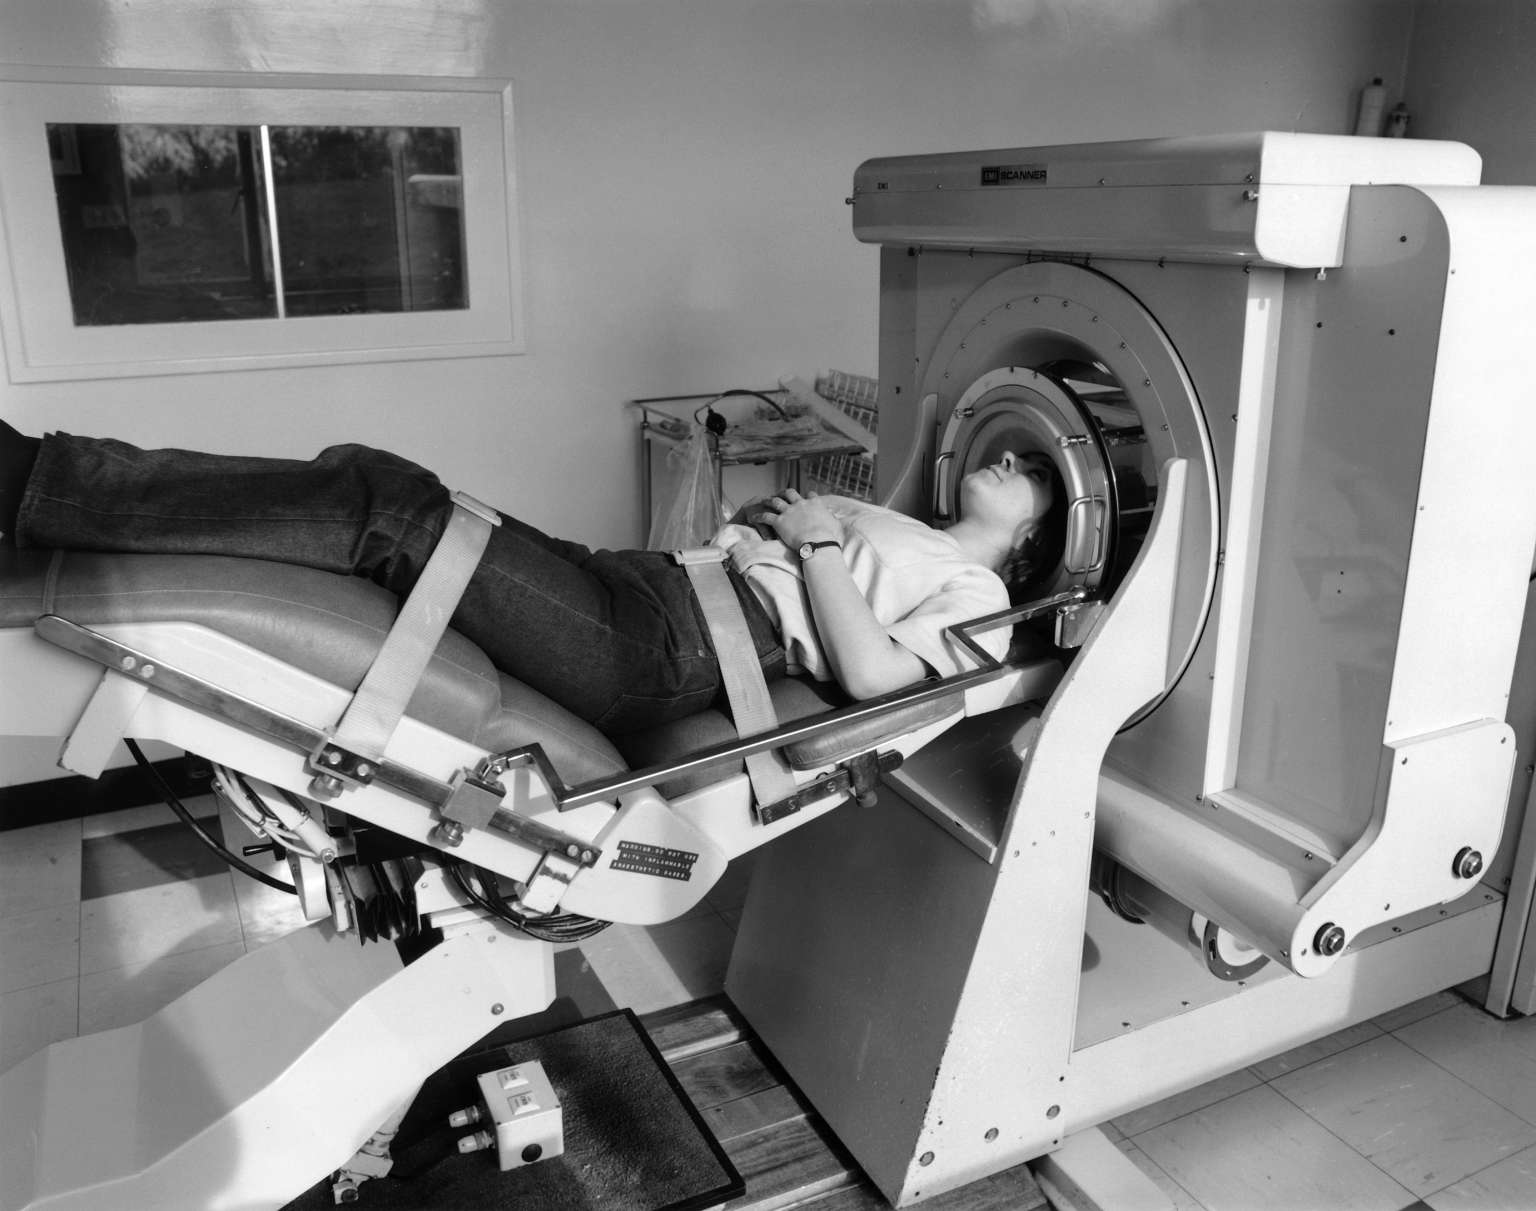
\includegraphics[width=10cm]{EMI_CT.png}
	\caption[EMI mark I]{EMI mark I sestrojený Godfrey Newbold Hounsfield v roce 1972}
\end{figure}
\null\\
CT přístroje je možné rozdělit do několika generací:
\begin{enumerate}
	\item generace - tato generace využívá tzv. Housofieldův systém, který byl použit i u přístroje EMI Mark I, snímkovací systém se v této generaci posouvá lineárně přes celou délku zkoumaného subjektu v dané rovině. Otočení je o zhruba 10$^\circ$ - 15$^\circ$. Zpracování snímků a vytvoření rekonstrukce trvalo cca 300 sec.
	\item generace - využívá stejný druh pohybu jako první generace, zmenšil se ovšem úghel mezi jednotlivými snímky na cca 3$^\circ$ - 10$^\circ$ a zvětšil se počet detektorů (až 60). Snížila se také doba rekonstrukce více než 10 a to na cca 20 sec.
	\item generace - tato generace je nejvíce využívanou variantou v současnosti. Rentgenka snímkuje objekt širokým snopcem záření za stálé rotace o 360$^\circ$. Použito je několik stovek detektorů (řádově 400-600) na protilehlé matici vůči zářiči. Snímkování se provádí po méně jak 1$^\circ$ a probíhá kontinuálně po celou dobu otořky.  \footnote[3]{Pokračováníma 3. generace je potom tzv. spirální (helikální) CT. To umožňuje postupný a plynulý posun stolu se zkoumaným objektem. Tato metoda byla poprvé použita v přístroji společnosti Bio-Imaging Research v roce 1986.}
	\item generace - Používá Rotující rentgenku, která opisuje celou kružnici záznam pak zajišťuje více než tisicovka stacionárním detekterů po obvodu. Problémem této generace je expozice okrajových detekterů, které jsou zasaženy rozptýleným a aodraženým zářením. 
	\item generace - tzv. nutační systém. ten se skládá z matice stacionárních detektorů a rotující rentgenky. Detektory se na základě pozice rentgenky vycylují z kolmice tak aby na ně paprsky dopadly kolmo. Tento systém umožňuje například rekonstrukci řezů v jiné než axiální rovině. \footnote[4]{V současné době (cca od roku 1999) vznikly i tzv. multi-slice CT. Tyto přístroje jsou vybaveny několika systémy detektorů uspořádaných do kruhu a umožňují tím pádem zísat více řezů v jednom okamžiku.Tímto způsobem ještě více urychlují vyšetření na druhou stranu stoupá jejich cena a náročnost údržby.}
	\item generace - tato generace jako zdroj záření používá elektronové dělo. Anoda je vlastně výsečí kolem čísti obvodu zkoumaného objektu a má několik ohnisek. Zařízení je buzeno současně na několika z ohniscích a detektory jsou umístěn do dvou prstenců okolo zkoumaného objektu. U této generace nedochází k žádnému pohybu. Zařízení je výše popsaným principem schopno snímkovat několik vrstev současně a to za extrémně krátkou dobu expozice, která se pohybuje okolo 50ms.
\end{enumerate}
\subsubsection{Princip CT}
Principem výpočetní tomografie, jak již bylo zmíněno výše je skládání celkového obrazu z mnoha jednotlivých snímků. U nejčastějšího typu CT přístrojů je rotuje rentgenka v gantře kolem pacienta a v pulzech trvajících 1-4ms vysílá vějířovitý rentgenový paprsek. Ten prochází snímkovaným objektem, kde je částečně absorbován. Po obvodu gántry jsou scintilační detektory, které zaznamenávají dopadající záření respektive míru jeho zeslabení. Tato informace je uložena do počítače a následně vyhodnocena. Obraz je potom informací o tom, jak jednotlivé voxely \footnote[3]{Voxel martix element - analogie pixelu v planárním obraze. Oproti dvojrozměrnému pixelu mají voxely ještě hloubku.}. Z pohledu medicíny je výsledkem výpočetní tomografie obraz pacienta v příčné (axiální) vrstvě, kdežto u rentgenovýh snímků vzniká obraz v frontální či sagitální vrstvě (v závislosti na poloze pacienta).\\
Absorbce rentgenového záření pro homogenní absorbér je dána následujícím vztahem:
\begin{equation}
 \centering
	I = I_{0}e^{-( \mu_{1}*x_{1} + \mu_{2}*x_{2} + ... + \mu_{y}*x_{y})}	
\end{equation}
Kde $ I_{0}$ je počáteční intezinta záření před průchodem zkoumaným objektem. $ \mu_{1}*x$ je pak součin lineárního koeficintu zeslabení $\mu$ a tloušťky homogenní části prostředí $x$. Výpočet zeslabení $I$ můžeme graficky znázornit následně:
\begin{figure}[h!]
 \centering
	\includegraphics[width=6cm]{zeslabeni_rtg_zar.png}
	\caption[Výpočet absorbce]{Výpočet zeslabení intentizi záření po prochodu absorbérem.}
\end{figure}
Nyní na jednoduchém proncipu můžeme vysvětlit na jednoduchém příkladu princip jakým je dopočítána informace pro výsledný obraz CT. Předpokládejme čtverce rozdělený na čtyři homogenní absorbéry charatkerizované zeslabením záření pro jednoduchost vyjádřeného $x_{1} - x_{4} $ s danými hodnotami. Tak jak je naznačeno na následujícím schématu:
\begin{figure}[h!]
 \centering
	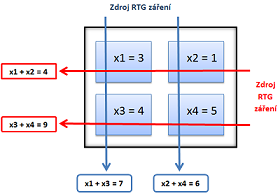
\includegraphics[width=6cm]{princip_CT.png}
	\caption[Princip výpočtu zeslabení voxelů]{Zjednodušený příklad principu výpočtu zeslabení jednotlivých voxelů}
\end{figure}
Hodnoty jednotlivých komponent $x_{1} - x_{4}$ jsou pro nás ovšem neznámou. Změřit je tedý možné jen zeslabení intentizity vždy v dané rovině (hodnoty v červených a modrých obdélnících). Díky těmto hodnotám jsme ale schopni sestavit 4 rovnice o 4 neznýámých:
\begin{equation}
 \centering
\begin{array}[h]{c}
	x_{1} + x_{2} = 4 \\
	x_{3} + x_{4} = 9 \\
	x_{1} + x_{3} = 7 \\
	x_{2} + x_{4} = 6
\end{array}
\end{equation}
Touto jednoduchou soustavou rovnic jsme pak schopni dopočítat jednotlivé parametry $x_{1} - x_{4}$. \\
Pokud se jedná o nehomogenní absorbér dostává rovnice (1) tento tvar:
\begin{equation}
 \centering
	I(x) = I_{0}(x)e^{-(\int\mu(x,y) dy) }
\end{equation}
Logaritmování tohoto vztahu dostaneme:
\begin{equation}
 \centering
\begin{array}[h!]{c}
	p(x) = -\left[\frac{I(x)}{I_{0}(x)}\right] \\
	p(x) = \int\mu (x,y) dy
\end{array}
\end{equation}
V praxi se ovšem vychází při řešení úlohy přiřazení správné hodnoty absorbce jednotlivým voxelům z tzv. Radonova transormace \footnote[5]{Autorem je Prof. Dr.phil. Johann Karl Gustav Radon narozen v Děčíne v roce 1887.} a zpětná Radonova transformace, což je integrální transformace spočívající v integrovýání funkce přes přímky. Při výpočtu CT obrazu se používá následující tvar:
\begin{equation}
 \centering
	p(r,\theta) = \int_{-\infty}^{\infty}\int_{-\infty}^{\infty} f(x,y) \delta(x cos\theta +y sin \theta - r)dx dy
\end{equation}
kde $f(x,y)$ reprezentuje $\mu (x,y) dy$ z rovnice (1), $r$ je pozice zdroje rentgenového záření a $\theta$ je úhel jeho natočení. Z tohoto vztahu je pak možné odvodit zpětnou Radonovu transformaci a s jejím použitím a využitím tzv. řezového teorému je pak možné získat dokonalý obraz pro všechny úhly. Radonova transformace se ovšem v praxi ukázala jako nestabilní a tak je v praxi nahrazena metodou filtrované projekce a Fourierova transformace.
\begin{figure}[ht!]
 \centering
	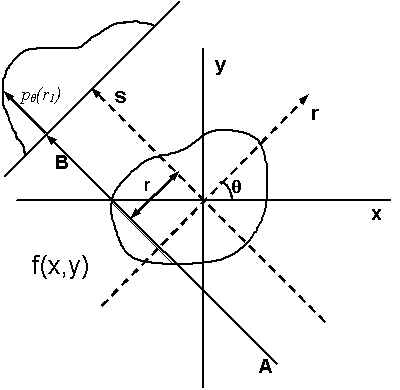
\includegraphics[width=6cm]{radonova_transformace.png}
	\caption[Radonova transformace]{Princip Radonovy transformace graficky}
\end{figure}
\subsubsection{Hounsfieldovy jednotky}
Hounsfieldova jednota (dále HU, někdy označované jako CT číslo) je denzintní jednotka vyjadřující míru absorpce jednoho voxelu vzhledem k refereční hodnotě absorbce vody (pro vodu HU = 0). Výpočet HU je definován následujícím vztahem:
\begin{equation}
 \centering
	HU = \frac{\mu -  \mu_{\omega}}{\mu_{\omega}}k
\end{equation}
Kde $k=10^3$ - je konstanta, $\mu$ - je koeficient zeslabení tkáně a $\mu_{\omega}$ - je koeficient zeslabení vody ( $ = 0,22cm^{-1}$). Ze vztahu (6) je patrné, že se HU je bezrozměrná veličina.\\
Rekonstruovaný CT obraz je nejčastěji zobrazován v odstínech šedi. Po provedení počítačových výpočtů je tak možné definovat rozsah zobrazovaných dat, právě rozsahem HU. Ten je pak přepoškálován a na vzniká tak grafická podoba CT snímku v odstínech šedi odpovídajících právě HU. Tímto je možné z naměřených dat analyzovat například pouze ty tkáně, na něž je vyšetření CT zaměřeno. Následující obrázek ukazuje vliv volby rozsahu na snímku plic:
\begin{figure}[ht!]
 \centering
	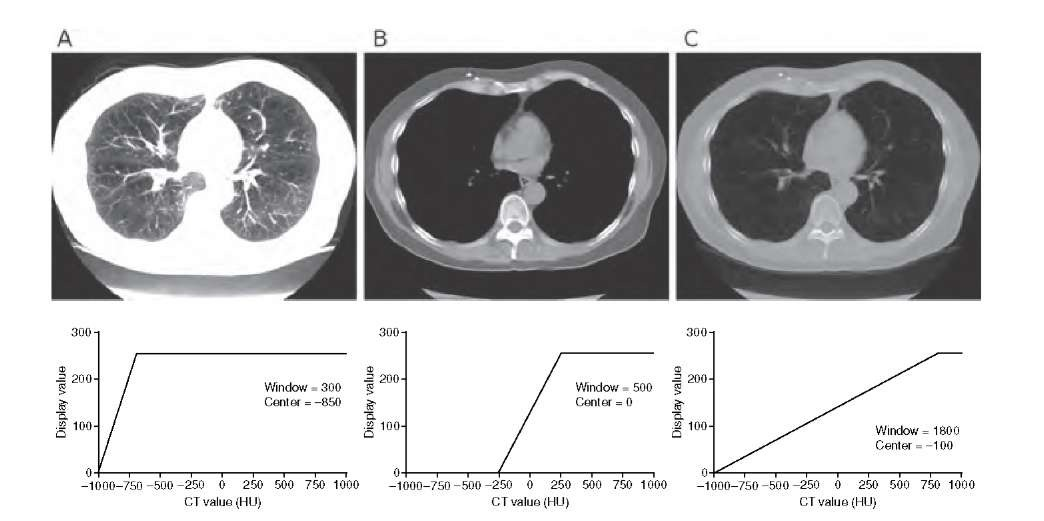
\includegraphics[width=10cm]{ruzna_HU.jpg}
	\caption[Nastavení rozsahu HU]{Nsatavení rozsahu zobrazeného HU pro CT snímek plic}
\end{figure}
V následující tabulce jsou pak zapsány přibližné hodnoty HU pro typické tkáně a orgány:
\begin{tabular}{c|c}
 \centering
\bfseries \bfseries Tkáň & \bfseries Densita HU\\
\hline \hline
vzduch                      & -1000\\
tuk                            & -50 - (-100)\\
voda                         & 0\\
likvor                         & 5\\
bílá hmota mozková  & 30\\
šedá hmota mozková& 34\\
krev                           & 47\\
játra                          & 40 - 60\\
svaly                         & 35 - 75\\
vazivové tkáně         & 60 - 90\\
chrupavka                 & 80 - 130 \\
kost                           & 1000 - 3000 
\end{tabular}
\captionof{table}{Orientační hodnoty HU}
\subsubsection{Mikro CT}
V této diplomové práci je jedním z cílů kombinovat data z Micro CT a klasického "makro" CT přístroje. V prvním zmíněném případě snímkování probíhá na Xradia MicroCT. Tento přístroj umožňuje skenovat vzorky do hnmotnosti 1kg a rozměru 100 mm. Rozlišovací schopnost je pod 1$\mu$  a velikost pixelu až 0,56$\mu$. Narozdíl od klasického CT microCT přístroje mají statický zářič i detektory a otáčí se přímo zkoumaný objekt. Snímkování pomocí těchto přístrojů také trvá výrazně delší dobu (standartně několik hodin).
\begin{figure}[ht!]
 \centering
	\includegraphics[width=10cm]{xradia.jpg}
	\caption[Micro CT Xradia]{Micro CT Xradia (MicroXCT-200) }
\end{figure}

\newpage
\listoffigures
\listoftables

\begin{thebibliography}{DUSO}
  \bibitem[1]{hugo} Jan Hugo:
    \emph{Velký lékařský slovník}. Maxdorf, Praha, 2015. ISBN: 978-80-7345-456-2 
  \bibitem[0]{medbio} Jozef ROSINA, Leoš NAVRÁTIL:
    \emph{Medicínská biofyzika}. Grada, Praha, 2005. ISBN: ISBN 80-247-1152-4
 \bibitem[0]{lekbio} Vojtěch MORNSTEIN, Ivo HRAZDIRA:
    \emph{Lékařská biofyzika a přístrojová technika}. Neptun, Brno, 2001. ISBN: 80-902896-1-4.
 \bibitem[0]{bak1} Renáta Chylíková:
    \emph{Výpočetní tomografie s vysokým rozlišením – jeho úloha a postavení v radiodiagnostice - Bakalářská práce}. Zdravotně sociální fakulta, Jihočeská univerzita v Českých Budějovicích, 2011.



   \bibitem[WikiSkripta]{WikiSkripta} WikiSkripta:
    \emph{Výpočetní tomografie a Hounsfieldovy jednotky}. \\
    \verb|https://www.wikiskripta.eu/w/V\%C3\%BDpo\%C4\%8Detn\%C3\%AD_tomografie_a_Hounsfieldovy_jednotky|
 \bibitem[Wikipedie]{Wikipedie} Wikipedie:
    \emph{Výpočetní tomografie}. \\
    \verb|https://cs.wikipedia.org/wiki/V\%C3\%BDpo\%C4\%8Detn\%C3\%AD_tomografie|
 \bibitem[what-when-how]{what-when-how} what-when-how In Depth Tutorials and Information:
    \emph{Gray-Scale Image Visualization}. \\
    \verb|http://what-when-how.com/biomedical-image-analysis/gray-scale-image-visualization-biomedical-image-analysis/|

\end{thebibliography}
  
%
\end{document}